%%
%% This is file `sample-manuscript.tex',
%% generated with the docstrip utility.
%%
%% The original source files were:
%%
%% samples.dtx (with options: `manuscript')
%% 
%% IMPORTANT NOTICE:
%% 
%% For the copyright see the source file.
%% 
%% Any modified versions of this file must be renamed
%% with new filenames distinct from sample-manuscript.tex.
%% 
%% For distribution of the original source see the terms
%% for copying and modification in the file samples.dtx.
%% 
%% This generated file may be distributed as long as the
%% original source files, as listed above, are part of the
%% same distribution. (The sources need not necessarily be
%% in the same archive or directory.)
%%
%% The first command in your LaTeX source must be the \documentclass command.
%%%% Small single column format, used for CIE, CSUR, DTRAP, JACM, JDIQ, JEA, JERIC, JETC, PACMCGIT, TAAS, TACCESS, TACO, TALG, TALLIP (formerly TALIP), TCPS, TDSCI, TEAC, TECS, TELO, THRI, TIIS, TIOT, TISSEC, TIST, TKDD, TMIS, TOCE, TOCHI, TOCL, TOCS, TOCT, TODAES, TODS, TOIS, TOIT, TOMACS, TOMM (formerly TOMCCAP), TOMPECS, TOMS, TOPC, TOPLAS, TOPS, TOS, TOSEM, TOSN, TQC, TRETS, TSAS, TSC, TSLP, TWEB.
% \documentclass[acmsmall]{acmart}

%%%% Large single column format, used for IMWUT, JOCCH, PACMPL, POMACS, TAP, PACMHCI
\documentclass[acmlarge,screen]{acmart}

%%%% Large double column format, used for TOG
%\documentclass[acmtog, authorversion]{acmart}

%%%% Generic manuscript mode


%%
%% \BibTeX command to typeset BibTeX logo in the docs
\AtBeginDocument{%
\providecommand\BibTeX{{%
\normalfont B\kern-0.5em{\scshape i\kern-0.25em b}\kern-0.8em\TeX}}}


%%
%% The majority of ACM publications use numbered citations and
%% references. The command \citestyle{authoryear} switches to the
%% "author year" style.
%%
%% If you are preparing content for an event
%% sponsored by ACM SIGGRAPH, you must use the "author year" style of
%% citations and references.
%% Uncommenting
%% the next command will enable that style.
%%\citestyle{acmauthoryear}

%%
%% end of the preamble, start of the body of the document source.
\begin{document}

%%
%% The "title" command has an optional parameter,
%% allowing the author to define a "short title" to be used in page headers.
\title{Designing a simple real time operating system for a ST Micro 32 bit processor}

%%
%% The "author" command and its associated commands are used to define
%% the authors and their affiliations.
%% Of note is the shared affiliation of the first two authors, and the
%% "authornote" and "authornotemark" commands
%% used to denote shared contribution to the research.

\author{Joseph Dobesh}
\affiliation{%
\institution{Candidate}
}
\email{10815159@uvu.edu}

\author{Frank Jones}
\affiliation{%
\institution{Advisor}
}
\email{FrankJ@uvu.edu} 
%%
%% By default, the full list of authors will be used in the page
%% headers. Often, this list is too long, and will overlap
%% other information printed in the page headers. This command allows
%% the author to define a more concise list
%% of authors' names for this purpose.
\renewcommand{\shortauthors}{Joseph Dobesh}

%%
%% The abstract is a short summary of the work to be presented in the
%% article.
\begin{abstract}
\textbf{Abstract - In model railroading, the hobbyist has two choices when it comes to controlling a railroad; buying off-the-shelf systems or designing a system from scratch. For someone with the ambition and time, designing a custom system yourself is more satisfying and can be a way to grow your skills. At the heart of such a system is the real time operating system (RTOS) which is the core of this project. It will hereafter be called the UVU RTOS or UTOS. UTOS utilizes a round robin preemptive context switching task manager. Additional features include mail services, pipelines, Ethernet, mutexing, limited file services and peripheral drivers. As is typical with other RTOS hosted applications, the user applications in this project are built into the kernel during compile time.}\\

\textbf{In this project I will be using model railroad applications to demonstrate the kernel functions. The railroad applications include control of locomotive speed and direction, track switching, and crossing gate control. This project can be easily expanded to include different scheduling methods, kernel functions, more elaborate file systems, extended network features, extended command line functions and more peripheral drivers.}
\end{abstract}

%%
%% Keywords. The author(s) should pick words that accurately describe
%% the work being presented. Separate the keywords with commas.
\keywords{STM32, RTOS, context switching, model railroad automation}

%%
%% This command processes the author and affiliation and title
%% information and builds the first part of the formatted document.
\maketitle

\section{Introduction}
Model railroading can be a fun and rewarding hobby. Not only can it provide hours of enjoyment, but can provide the hobbyist with opportunities to learn new skills, including electronics and programming. Some hobbyists choose to control their railroad by buying off-the-shelf systems. Such systems often use the National Model Railroad Association (NMRA) Digital Command Control (DCC) standard\cite{DCC01}. This standard allows different manufacturers to create products that will work with one another. Controllers and modules are strung together on the DCC bus allowing the operator to control everything from the speed of multiple locomotives to sound effects on the layout. Building a railroad using these off-the-shelf systems can be expensive and designing a custom system yourself can be more satisfying and cost effective.\\

In this project I have designed and implemented a railroad control system built upon a simple real-time operating system (RTOS). I have called this RTOS the UVU real time operating system, or UTOS. The UTOS differs from typical operating systems in that it has a smaller image footprint, has less features, and is meant to run on embedded microcontrollers.\\

There are at least three advantages to running UTOS on your embedded system. One is that the kernel does not have a lot of overhead. This allows more time for the user applications to run. Many times applications are controlling hardware that require a near instantaneous response from the controller. Any delay could be catastrophic. Another advantage of running UTOS is that most microcontrollers have limited memory space, both in program memory and RAM. UTOS has a smaller kernel than other off the shelf operating systems. This makes more efficient use of memory space, both FLASH and RAM. Lastly, UTOS will have features and drivers that do not come standard in a typical PC based operating system, such as Pulse Width Modulation (PWM) and General Purpose Input/Output (GPIO).\\

One of the defining aspects of UTOS is its round-robin preemptive context switching task schedular. Other additional features are, but not limited to, soft timers, a mail system, FIFOs/pipelines, mutex functionality and serial drivers. In the interest of time and code size a built-in TCP/IP stack was used with HTTP CGI and SSI functionality. This stack was included with the STM32 Cube IDE. Another feature that I have added is command line functionality that can navigate a FAT32 file system on an SD card, run some of the user applications, and test some of the kernel functions. Most of this project was written in C except for the HTML pages that the operator uses to remotely control the railroad. One page is dedicated to locomotive speed control and direction. One page monitors crossing gate status of the selected crossing gate. And one page monitors the loopback track switch along with the track voltage polarity with the ability to override the switch position. UTOS runs on the ST Micro NUCLEO-F429ZI evaluation board which uses the ST32F429ZI 32-bit ARM Cortex-M4 microcontroller.\\

Along with the standard operating system features that I have included, I have also added drivers for supporting hardware that is unique to this project. One is a driver for communicating on the Modbus control network. Modbus is a open-source communication protocol for communicating with industrial controls. I have used these controllers to interface the user applications with the model railroad hardware. The Modbus protocol documentation can be found at numerous sources on the web.\\

I have developed three model railroad applications that demonstrate and validate most of the features of UTOS. The first is the speed control task which controls the speed and direction of the locomotive. This task can be controlled from either an HTML page or the command line prompt. There is also a crossing gate control task which monitors the rail road crossings and lowers the crossing gates when a train approaches. The third task is a loopback control that controls polarity and switch direction of a loop when a locomotive is operating within the loop.
\section{Hardware Architecture and Implementation}
This project utilizes the ST Microelectronics Nucleo-F426ZI evaluation board which features the ST Micro ST32F429 ARM Cortex-M4 microcontroller\cite{Nucleo02}. This evaluation board has many peripherals such as an Ethernet controller, SPI and UART ports, standard I/O and PWM controllers. All of which have been implemented in this project. See Figure 1. The Laptop or PC in the figure is optional and is only used to program the Nucleo, do debugging, testing and provide a terminal for the command prompt feature.\\
\begin{figure}[H]
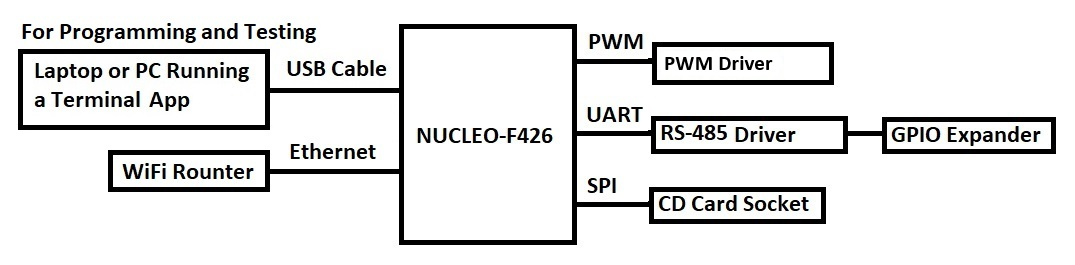
\includegraphics[scale=0.5]{UpperLevel.jpg}
\caption{Upper Level Diagram}
\label{Fig 1: Upper Level Diagram}
\end{figure}
There are also other peripheral devices required for controlling the railroad layout, hereafter called the layout. They are listed as follows:\\
\begin{enumerate}
\item (Qty 1) RS-485 Driver, Garosa da22f385-347a-434e-bac3-74f94ecb2d2e
\item (Qty 1) PWM Driver, Anmbest MD114
\item (Qty 1) Modbus Digital I/O expansion module. 16 channels, Eletechsup N4D3E16
\item (Qty 2) Switch Machines, Walthers 942-101
\item (Qty 7) Digital IR Sensors, Iowa Scaled Engineering CKT-IRSENSE
\item (Qty 2) 12VDC 10A DPDT relays, YYUAN MY2NJ
\item (Qty 1) 12VDC 10A Power Supply, Alitove 12V-10A-T
\item (Qty 1) Multiple Output Power Supply (3.3, 5, 12, Adj), NYSUZHOUJI t8uo9nhgpe\\
\end{enumerate}
The following figures show simplified block diagrams of each of the features utilized in this project with an explanation of their use in the layout.\\
Figure 2 shows the power supply arrangement. The 12 VDC power supply is needed to supply power to the locomotives running on the layout and also supplies power to the other low voltage supplies. These supplies power the devices used in controlling the layout.
\begin{figure}[H]
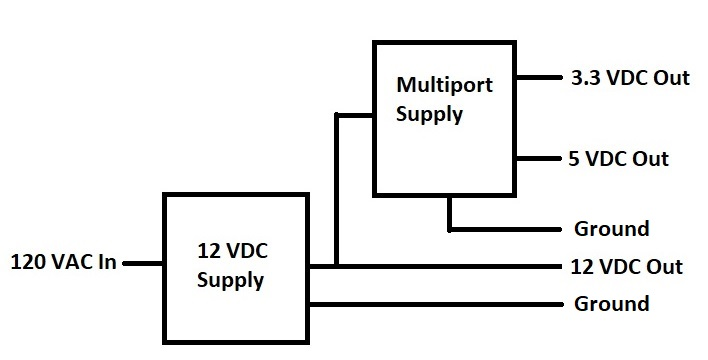
\includegraphics[scale=0.5]{Power Supplies.jpg}
\caption{Power Supplies}
\label{Fig 2: Power Supplies}
\end{figure}
Figure 3 shows the wiring diagram for the PWM driver. This driver provides the necessary current and voltage required for controlling the speed of the locomotives. An additional diode is supplied to reduce spikes during switching.
\begin{figure}[H]
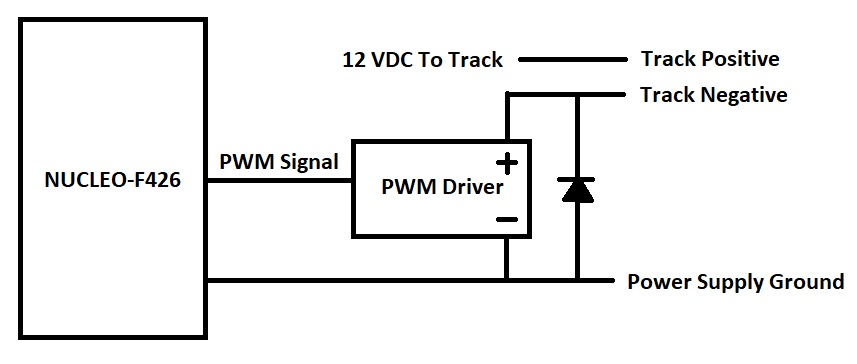
\includegraphics[scale=0.5]{PWM.jpg}
\caption{PWM Circuit}
\label{Fig 3: PWM Circuit}
\end{figure}
Figure 4 shows the RS-485 driver. The driver incorporates the Maxim MAX1787 RS-485 transceiver\cite{MAX1487}. This driver connects to communication lines coming from the Nucleo UART Tx and Rx lines. The DE and /RE control lines are tied together and connected to a GPIO port. This wiring arrangement allows the RX-485 driver to work as a half-duplex bus. The DE/RE line switches the driver from Rx mode to Tx mode.
\begin{figure}[H]
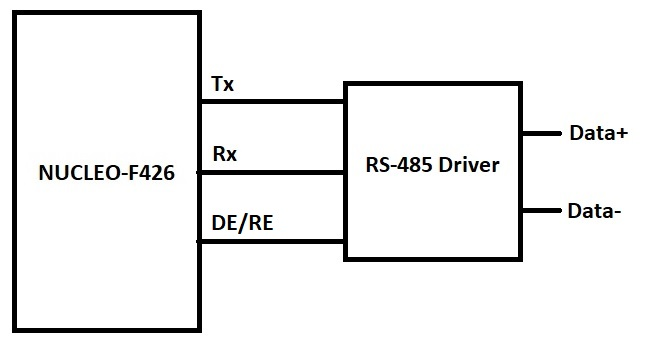
\includegraphics[scale=0.5]{RS-485.jpg}
\caption{RS-485 Driver}
\label{Fig 4: RS-485 Driver}
\end{figure}
Figure 5 presents the connections to the Modbus I/O expansion module\cite{Eletechsup01}. This module communicates with the Nucleo through the RS-485 bus. It also provides inputs for the IR sensors on the layout and outputs for the polarity relays and switch motor. The IR sensors detect trains passing over them\cite{ISE01}\cite{ise02}. The relays control the polarity of the voltage going to the locomotives. The switch machines control the direction of the track switches and the crossing gates on the layout\cite{Walthers01}. 
\begin{figure}[H]
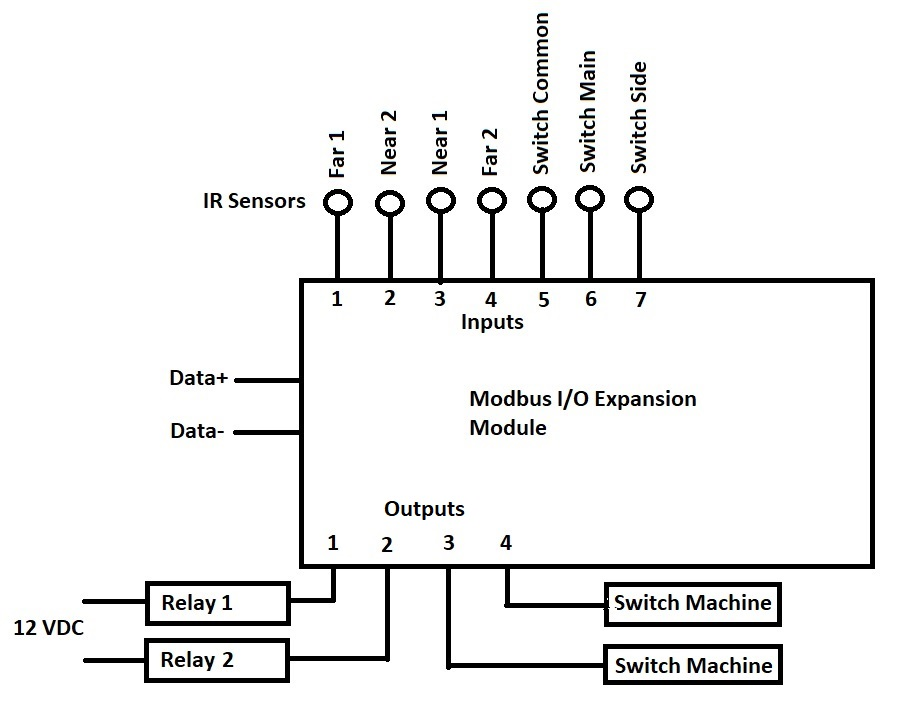
\includegraphics[scale=0.5]{Module.jpg}
\caption{Modbus I/O Expansion Module}
\label{Fig 5: Modbus I/O Expansion Module}
\end{figure}
\section{Software Architecture and Implementation}
In this section I discuss the design and implementation of the UVU Real Time Operating System (UTOS). I start by explaining the built-in features of the ARM hardware that make creating a preemptive context switching scheduler much simpler. I then go into the design of the kernel itself and the additional features that make designing applications easier. Finally, I explain the example model railroad applications themselves.\\
\subsection{Task Manager/Kernel}
The core of the UTOS is the round-robin preemptive context switching schedular. This scheduler was initially implemented as a simple cooperative task manager. A cooperative task manager relies on tasks that willingly give up CPU time when they are in a waiting or in an idle state. One of the drawbacks of this approach is that very large tasks can dominate a large amount of CPU time. Additionally, the programmer would have to make sure to write interruptions periodically throughout the code, which could make it complicated and bloated. Still, such a schedular is easy to implement and so initially, I used this technique to develop and test hardware drivers before moving on to a more complicated kernel. I will not go into further detail on the cooperative switcher because the ultimate goal was to create a preemptive context switcher.\\

The round-robin preemptive context switcher interrupts a task periodically via a timer interrupt. The timer has a constant value and each task is given equal time to run. See Figure 6.\\
\begin{figure}[H]
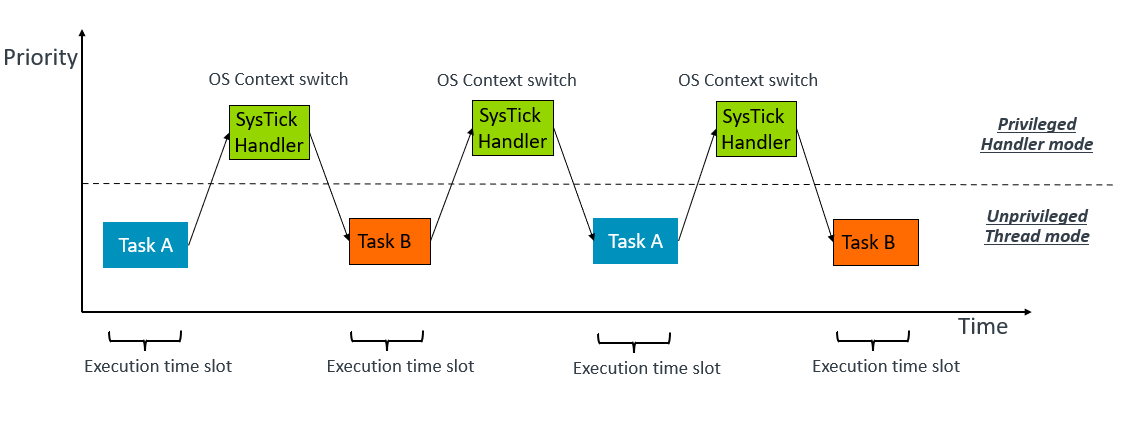
\includegraphics[scale=0.75]{PendSV.png}
\caption{Preemptive Context Switcher}
\label{Fig 6: Preemptive Context Switcher}
\end{figure}
\subsubsection{The ARM Processor}
The ARM family of processors have several attributes that make them attractive for building your own RTOS. To begin with, there are 16 dedicated exception vectors that help in creating a scheduler. See Table 1.
\begin{table}[H]
\caption{ARM Exception Table}
\centering
\begin{tabular}{c c} 
\hline
Exception Number & Exception \\
\hline
1 & Reset \\
2 & NMI \\
3 & HardFault\\
4 & MemManage \\
5 & BusFault \\
6 & UsageFault\\
7-10 & Reserved\\
11 & SVCall\\
12 & DebugMonitor\\
13 & Reserved\\
14 & PendSV\\
15 & SysTick\\
\hline
\end{tabular} 
\end{table}
The two exceptions that are most relevant to scheduling are the SysTick and PendSV exceptions. The SysTick exception can be used as a simple tick timer (and as such I use this feature to track the blinking time of the Heartbeat LEDs talked about below), but it can also be used as a preemptive timer for the context switcher. One method of doing so is to count the number of ticks until the switching value is reached and then have the SysTick routine set the ICSR bit in the SCB register. This triggers the PendSV exception. After the register is set, the switching counter is set back to zero. More information on this strategy can be found at the ARM website.\cite{ARM01}. See Figure 7.\\
\begin{figure}[H]
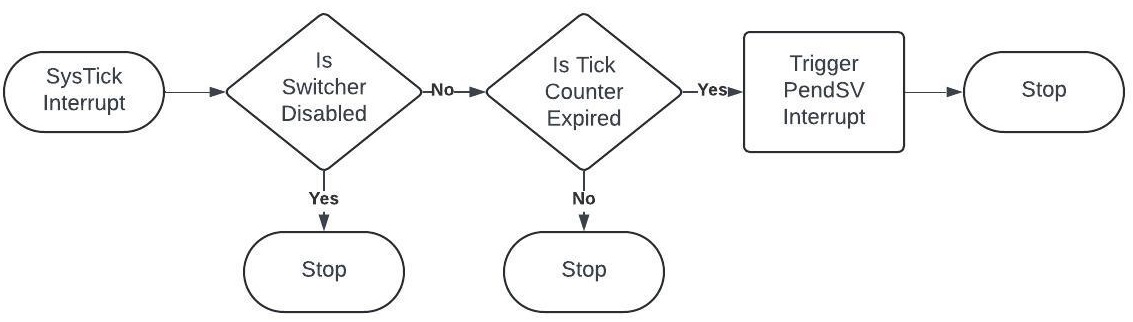
\includegraphics[scale=0.5]{SysTick2.jpg}
\caption{SysTick Routine}
\label{Fig 7: SysTick Routine}
\end{figure}
When the PendSV exception is triggered, It begins by saving all the context registers to the Process Control Block (PCB). Each task is assigned a PCB. The PCB is a structure that holds information about the task and also a pointer to the stack where the context registers are saved. More will said about the PCB below. After the context registers are saved, the switching routine in the kernel is called. This routine saves the PCB onto a queue and pulls the next PCB from the queue. Upon returning from this routine, the context register values are copied from the PCB into the context registers and then the PendSV exception returns. See Figure 8.\\
\begin{figure}[H]
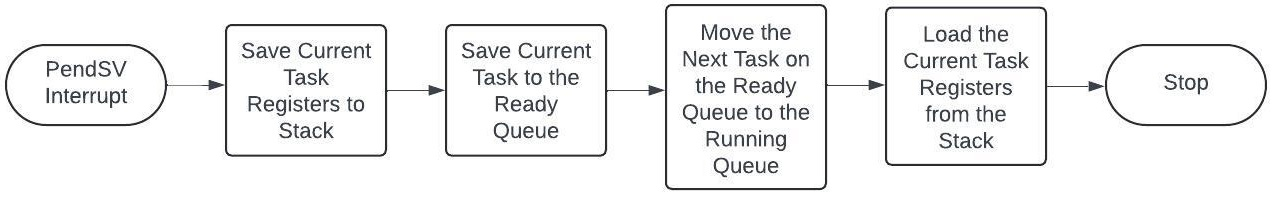
\includegraphics[scale=0.5]{PendSV2.jpg}
\caption{PendSV Routine}
\label{Fig 8: PendSV Routine}
\end{figure}
\subsubsection{Kernel Init}
The STM32 Family of processors come with a vast hardware interface library. I will make use of these libraries in the project. Most of the libraries are initialized in main before the kernel code is called. There is an endless while loop in main where the kernel is called. The kernel call never returns. When the kernel task is called, it first initializes any variables used in the running of the kernel, then it initializes any kernel modules, such as the mail and SD card modules. See Figure 9.\\ 
\begin{figure}[H]
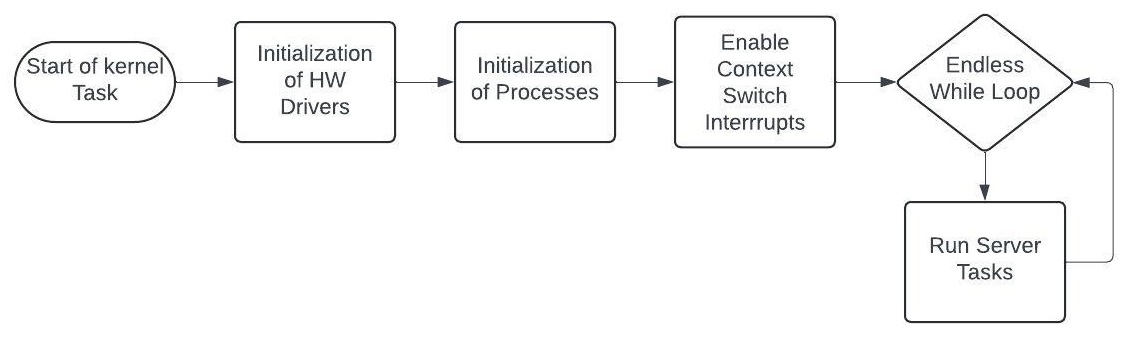
\includegraphics[scale=0.5]{KernelInit2.jpg}
\caption{Kernel Init}
\label{Fig 9: Kernel Init}
\end{figure}
The first step in kernel initialization is to setup the hardware drivers. In the next step, the kernel allocates a PCB for each task, initializes it, and places it onto the Ready Queue. The PCB structure holds critical information for each task, including a pointer to its dedicated stack and the function pointer to the task itself. For the Cortext-M4, the stack pointer must be the first element in the PCB structure and it must be the width of the Stack Pointer (SP) register. In our case, 32 bits.\\
Once the PCB has been initialized, the dedicated stack is initialized with default values for each saved register. Finally, a pointer to the PCB is pushed into the ready queue. Once each task is initialized and the PCBs are pushed onto the ready queue, the kernel enables the switcher interrupts, and enters its own endless loop.\\
The first tasks that are pushed onto the ready queue are kernel related tasks. This gives them a chance to run before any of the user tasks. Needless to say, they must be initialized so that if the user tasks need to interact with them, they will function normally.\\
As mentioned above, when the PendSV exception fires, it saves context registers and then calls the context switching routine. This routine is part of the kernel. The routine starts by pulling the current task PCB pointer value from the current task pointer variable and places it back on the pending task queue. Next it pulls the pending task PCB from the front of the queue and copies it on to the current task value. It then returns to the PendSV routine.\\
\subsection{UTOS Modules}
This section describes the kernel modules that are not part of the context switcher. These modules make it easier for applications to interact with the kernel, each other and any common resources. There are also modules that are part of the user interface that allow access to the kernel and the applications. I make extensive use of the book Operating System Concepts for ideas on how to construct these modules\cite{Silberschatz13}. The STM32CubeIDE comes with built in libraries that make it easier to interact with the hardware. I also made good use of these libraries\cite{HALManual01}.
\subsubsection{Heartbeat Tasks}
The heartbeat tasks are simple tasks that blink the red and blue LEDs every 1 second. This is to indicate to the user that the system is running and not locked up in some way.\\
\subsubsection{Mailbox Task}
The Mailbox task is a post office. The module allows a process to send messages to more than one destination. It is protocol independent, which means the messages can be of any protocol to communicate between users. The end users need only know the protocol it will receive from the source. All users need to register a mailbox. If a source mailbox sends a message to an unregistered mailbox, the source will be notified. Every registered mailbox will have its own memory allocation. If the mailbox gets full, the oldest mail will be discarded. The job of the task is to gather mail from source mailboxes and redistribute the mail to the destination mailboxes. See Figure 10. It also has the job of cleaning up any mailboxes that are unregistered. The mailbox is not an efficient tool for steaming data from one task to another, but is useful for sending large messages periodically. See pipeline FIFO below.\\
\begin{figure}[H]
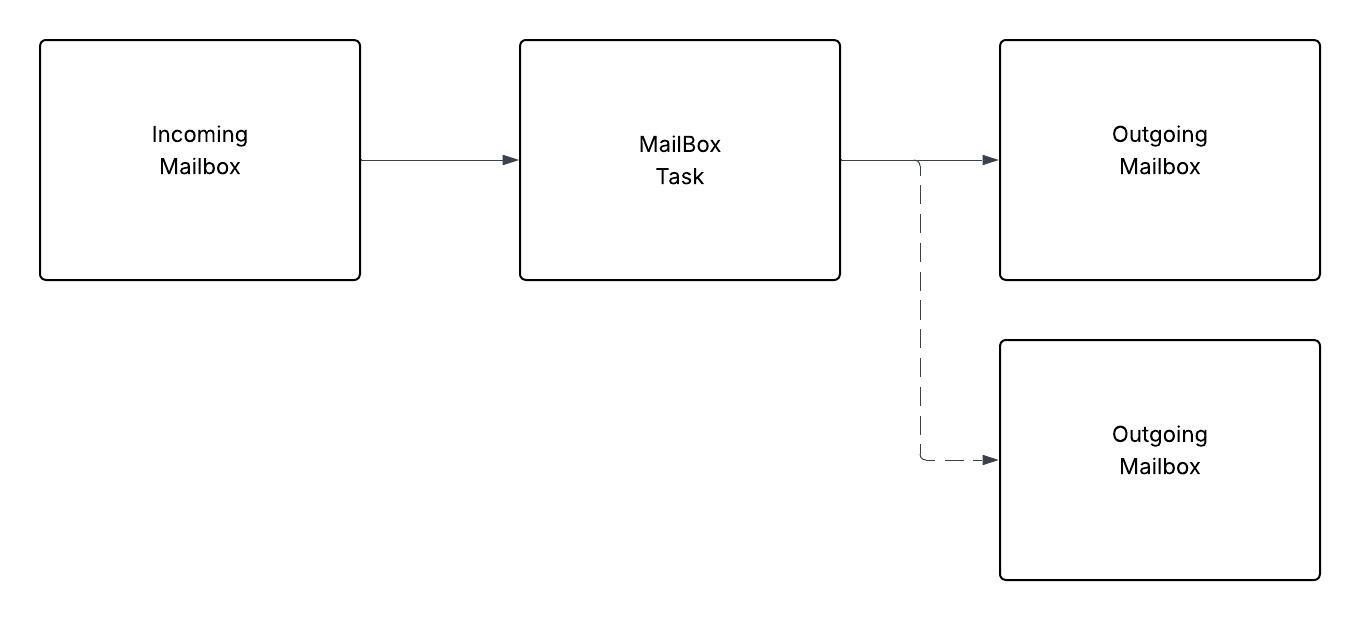
\includegraphics[scale=0.35]{Mailbox.jpeg}
\caption{Mailbox}
\label{Fig 10: Mailbox}
\end{figure}
\subsubsection{Command Prompt Task}
The Command Prompt task is intended as a testing and debugging tool. The user can type commands to navigate the SD card, set and get the RTC date and time or run functional tests of the system.\\
There are four menus to select from in the main menu. Hitting the Enter key or typing help in the main menu displays a help for selecting a sub menu. The command prompt is accessed via a UART port in the evaluation board's USB connector. This connector also acts as the programming and debugging port. The user can use a terminal app, like Tera Term, configured as 115200-8-None-1-None to communicate with the controller. Most of the menus are self-explanatory. For more information, see the User's Manual section at the end of this document.
\subsubsection{Soft Timer Module}
The SoftTimers module is not a task in the sense that was discussed above. It is fully interrupt driven and does not have a task loop. It is meant to supply the different processes access to timers without having to access hardware. The user first registers with the module and if there is an available timer a timer ID is returned. Every time a process desires access the timer from this point, it needs to use its timer ID. The user has the choice of configuring the timer in two ways; they can configure it as a one-shot timer where the timer does not reset itself when the time expires or it can be set as continuous where the timer resets to a preconfigured time every time it expires. The user has the choice of passing a callback function pointer to the timer so that when the timer expires, this function is called, or the user can check the timer manually to see if it has expired.\\
Because the callback function is called as part of soft timer interrupt routine, there is nothing in the timer to prevent the callback function from running forever. The callback function should be designed as any other interrupt routine. There should not be any endless loops in the callback function and the call back function should be as short as possible. The best operation of the callback function would be to set some parameters and return and let a task do any processing on those parameters.\\
Once a process has finished using the timer, it should release the timer by passing the timer ID into the release function. This is highly recommended as the number of soft timers is limited to 8. The soft timers are based on a single hardware timer that fires an interrupt every 10 milliseconds.
\subsubsection{Pipeline/FIFO}
This module is a merger of pipelines and FIFOs according to the strict definitions. It is more of a pipeline because it does not treat the data buffer as a file. It can pass data within processes or between processes. Also, it can only pass data one way between a single point to another single point. An origin user begins by registering with the pipeline by giving it an unique ID. Part of registering a pipeline involves allocating memory. The destination user need not register, but they do need to know the ID of the sender. The sender passes data on the pipeline and the destination pulls the data off. Once the pipeline is not needed, the sender needs to release the pipeline and return it to the pipeline pool. The receiver should never release the pipeline
\subsubsection{Mutex Module}
The mutex module is meant to protect resources from being accessed by competing tasks. There is a mutex designator assigned to each resource that may be shared by tasks. Examples are the RS485 port buffers and the SD card. There are three types of blocking functions. The MutexSpinlock method will hold the task in an idle state indefinitely until the block is released by another task. At this point the waiting task will have the block. The MutexWait method will immediately return FALSE if the resource is blocked, otherwise it will return TRUE after grabbing the block. The MutexWaitTime method waits a specified amount of time before returning FALSE if the mutex remains blocked. If the block is released by another task before the timer expires, the block is grabbed by the waiting task and the method returns TRUE. Once a task is done using the resource it must call the MutexRelease method.
\subsubsection{Server Stack}
Initially, I was going to write my own stack and server to gain more experience with networking. In the interest of time and code size, I decided to instead use the LwIP stack that is included with the STM32 Cube IDE. Along with the stack there are also application layer options that include Common Gateway Interface and Server Side Includes. DHCP was disabled and a static IP address of 192.168.1.111 was assigned. See Figure 11.\\

Server Side Includes (SSI): This interface allows the HTTPD application layer to interface with the apps running on the controller and receives information from an application and displays it on a HTML page.\\

Common Gateway Interface (CGI): This interface allows the HTTPD application layer to interface with the apps running on the controller and sends information from a HTML page to the application.\\
\begin{figure}[H]
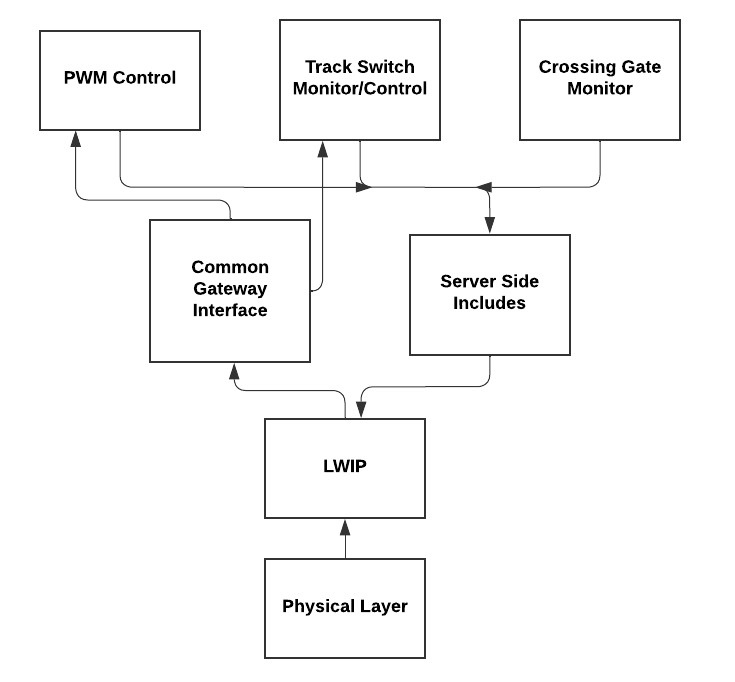
\includegraphics[scale=0.5]{ServerStack.jpg}
\caption{Server Stack}
\label{Fig 11: Server Stack}
\end{figure}
\subsubsection{File System Stack}
The file system stack sets up the SD Card for reading files. All files are in the root directory, which is typical in embedded systems. In the command prompt menu, the user can access the files by using the commands: ls - to list the files and cat - to print the files to the screen\cite{Axelson06}.
\subsubsection{Modbus/RS485 Drivers}
These low level hardware drivers create an interface for communicating with the Modbus hardware. The Modbus driver assembles messages that are then loaded into a UART send buffer and are clocked out by the hardware. Incoming messages fire an interrupt which pulls bytes from a UART input buffer and places them into a circular buffer. The Modbus parser then retrieves the message from the buffer and saves pertinent data from the message. The serial settings for Modbus are 9600-8-None-1-None.
\subsubsection{Real Time Clock (RTC)}
Support for the built-in RTC is included in the STM32 HAL libraries\cite{HALManual01}. It just needed to be set up in the STM32 CubeMX tool. I added the ability to get and set time and date in the command prompt menu.
\subsubsection{Watchdog Timer}
Support for the built-in Watchdog Timer (WDG) is included in the STM32 HAL libraries\cite{HALManual01}. Petting the dog happens in the tick timer interrupt. This way if the interrupts for the context switch ever get disabled by a task (which should never happen), the system will reset. This also protects from any unintended endless loops in places like the soft timer interrupt callback routines.
\subsection{User Applications}
This project includes three sample user applications. They are discussed in the fallowing subsections.
\subsubsection{Locomotive Speed Control}
The speed control application is designed to control the speed of the locomotive. It does this by controlling voltage to the tracks using the pulse width modulation (PWM) hardware on the STM32 processor. This signal is fed into a Power MOSFET to step up the voltage and current of the signal. The pulse width is divided into increments of 100, zero being off and 100 being full on. The average voltage can be changed by controlling the duty cycle of the signal. This example demonstrates an application that does not require any built-in UTOS task. The speed can be controlled from the web page or the command prompt.\\
There are few UTOS features that are used here. The Server Stack and the Command Prompt are used to adjust the speed.
\subsubsection{Crossing Gate Control}
The Crossing Gate Control application monitors four sensors that detect the approach of a train. There are two near sensors and two far sensors. The gates are lowered when a far sensor detects a train. See Figure 12.
\begin{center}
\begin{figure}[H]
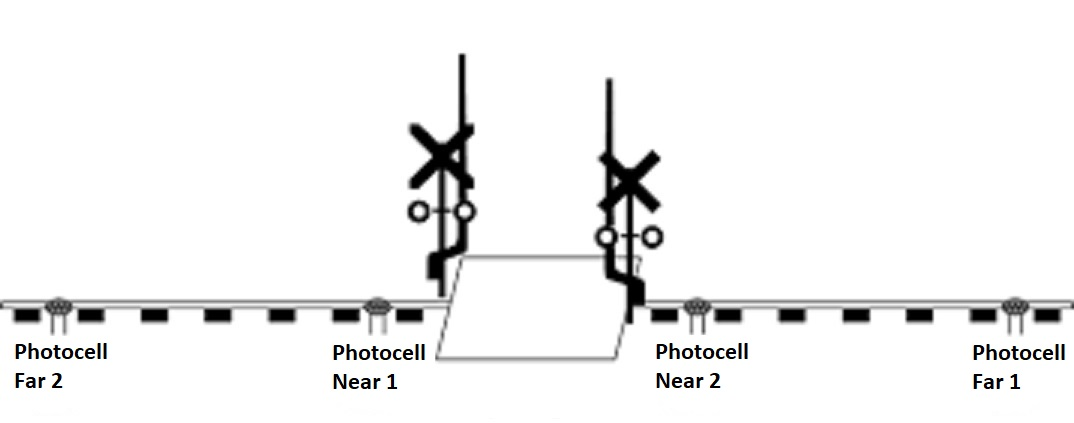
\includegraphics[width=80mm,scale=0.8]{Crossing Gate Image.jpg }
\caption{Crossing Gate Image}
\label{Fig 12: Crossing Gate Image}
\end{figure}
\end{center}
The application uses a state machine to progress through the sequence of sensor detections. When the matching near sensor detects the train, the application moves on to the next state. The gates will remain lowered until the near sensor and the matching far sensor have cleared. The state machine returns to the idle state when all sensors have cleared. See Figure 13. The sensors are interfaced with the controller by a Modbus I/O expansion module and must be polled on a regular basis. The gate motor is controlled by the same Modbus I/O expansion module.\\
The Crossing Gate control uses a number of UTOS tasks. A Soft Timer is used trigger a periodic poll of the gate sensors. The Pipeline is used to transfer data back and forth from the Modbus task. The Modbus task communicates commands to the crossing gate hardware. The Server Stack is used to monitor the status of the crossing gate.
\begin{center}
\begin{figure}[H]
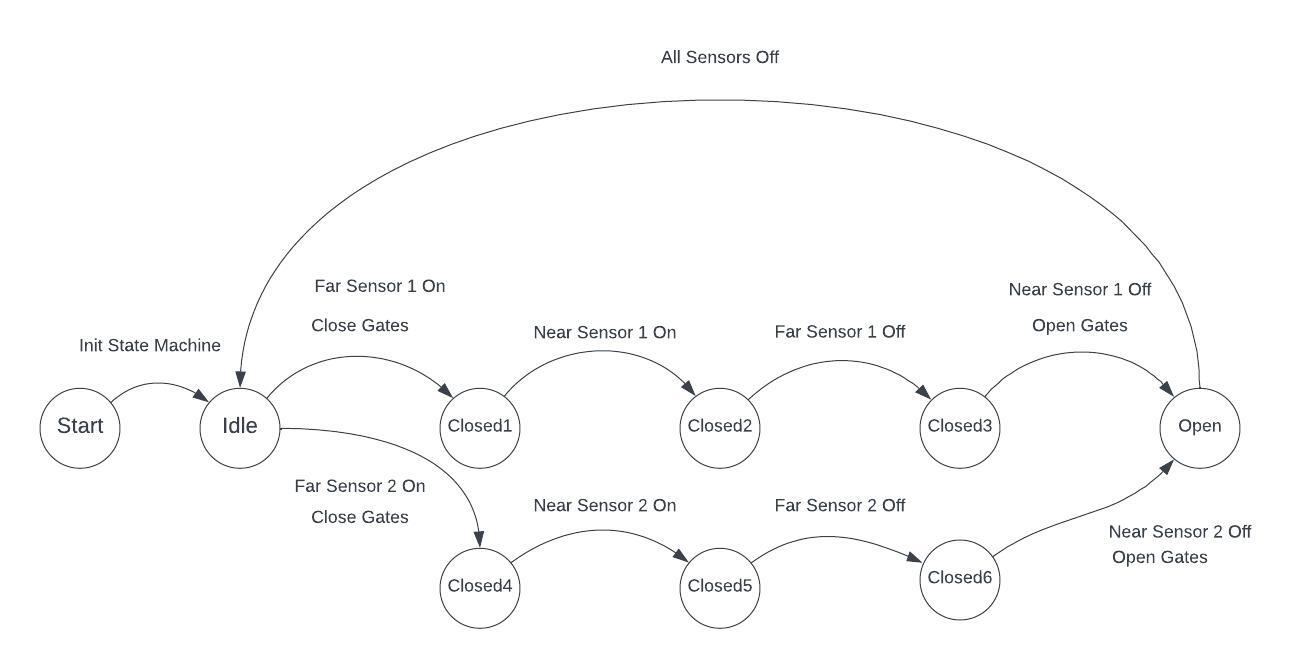
\includegraphics[width=\linewidth]{Gate Control State Machine.jpeg }
\caption{Gate Control State Machine}
\label{Fig 13: Gate Control State Machine}
\end{figure}
\end{center}
\subsubsection{Crossover Switch And Polarity Control}
The Crossover Switch and Polarity Control application monitors a crossover track switch and the track voltage polarity to make sure that there are no conditions where a possible derailment could happen. This can happen in two ways. One is when a train tries to pass through a track switch where the switch is closed against it. Think of a switch as a 'Y'. When a train is approaching from the base of the 'Y', it has two possibilities for a direction of travel. Thus, there are no chances for derailment. But, if the train is approaching from one of the branches of the 'Y', the switch must be in the position where that branch is selected. If not, there is a very good chance for derailment. In this case the controller detects the approach of a train in the branch and if the switch is closed against it, it will open the switch automatically. See Figure 14. There are track switches that will give way when the switch is closed against the oncoming train. This controller assumes that standard track switches are installed.
\begin{center}
\begin{figure}[H]
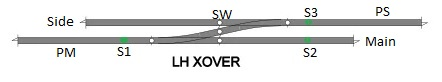
\includegraphics[width=\linewidth]{Crossover.jpg }
\caption{Crossover Switch}
\label{Fig 14: Crossover Switch}
\end{figure}
\end{center}
The second derailment condition happens when the train is approaching the track switch from the base of the 'Y' and the switch is closed. This means the train is being switched over to the side track. Normally, this would be OK if the side track voltage polarity matched that of the main track. If the side track's voltage polarity does not match that of the main track, the locomotive will be suddenly be thrown into reverse. The momentum of the cars will push against the locomotive and cause the train to pancake. The controller monitors the switch position and the voltage polarity of both tracks and makes sure the adjoining track has the same polarity. This truth table in Figure 15 shows the conditions on which polarity and switch position controlled. 
\begin{center}
\begin{figure}[H]
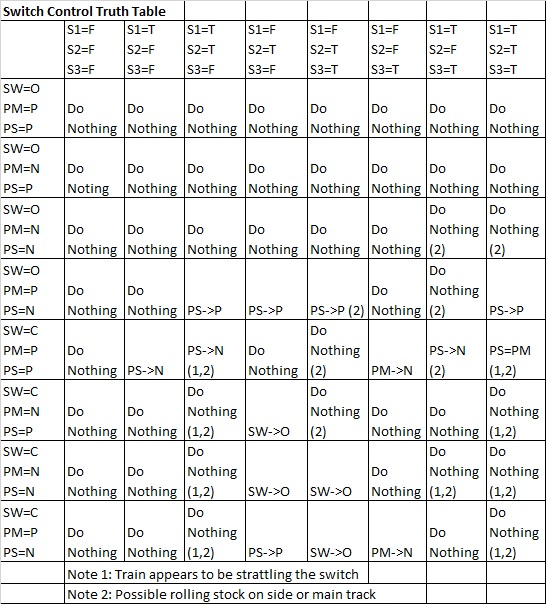
\includegraphics[width=60mm,scale=0.6]{TruthTable.jpg }
\caption{Crossover Switch TruthTable}
\label{Fig 15: Crossover Switch Truth Table}
\end{figure}
\end{center}
The UTOS modules used in the Crossover Switch control are the Soft Timers, The Pipelines, the Modbus task and the Server Stack. The Soft Timer is used trigger a periodic poll of the track switch sensors. The Pipeline is used to transfer data back and forth from the Modbus task. The Modbus task communicates commands to the crossover switch hardware. The Server Stack is used to monitor the status of the crossover switch and to override the switch motors and polarity relays.
\section{Project Results}
The main goal of this project was to create a round robin preemptive context switching operating system. Although the concepts were easy to understand, implementing them took more time than I anticipated. A number of tasks were also created that ran on the operating system and were meant to test and utilize the different OS features.\\
\subsection{Completed Features}
There were two types of tasks, those that tested the context switcher and those that served a purpose on the model railroad layout. There were two simple test tasks, each blinked an LED. The command prompt could also be considered an OS test task, but it was mainly meant to be a way to test hardware.\\
The user tasks, or railroad tasks, are the speed control, crossing gate controller and the crossover switch controller.\\
Below is a list of features that were completed in the project. Some of these features were outlined in the project proposal. Some were added later as they were advantageous to the project. I felt this was acceptable because I was using the Agile project management methodology from the beginning.
\begin{enumerate}
\item Time Interrupt Context Switching Operating System
\item Two heartbeat tasks that blinked LEDs
\item Command Prompt Task
\item Soft Timer Module
\item Pipeline/FIFO Module
\item Mailbox Module/Task
\item Mutex Module
\item TCP-IP Stack/Server
\item PWM Locomotive Speed Control
\item Crossing Gate Control Task
\item Track Switch Control Task
\item RTC - Real Time Clock
\item WDT - Watch Dog Timer interrupt
\end{enumerate}
\subsection{Deleted Features}
The following features that were mentioned in the proposal were removed from the project because they were deemed unnecessary to demonstrate the UTOS. They also did not add value to the railroad applications or they were redundant. Meaning other features did a better job.\\
\begin{enumerate}
\item Keypad - Most anything that can be entered on the keypad, can be done from the command prompt or on the web page. See Future Projects to see more replacements for this feature.
\item LED Character Display - Most anything that can be displayed on the LED Display, can be displayed from the command prompt or on the web page. See Future Projects to see more replacements for this feature.
\item Health Monitors - Temperature and humidity sensors do very littler to demonstrate the operation of the UTOS and are not needed on a model railroad layout.
\item Push Buttons - Most anything that can be done by a push button, can be done from the command prompt or on the web page. See Future Projects to see more replacements for this feature.
\end{enumerate}
\subsection{Difficulties}
For the longest time I was having trouble debugging the context switching routine. I thought it had something to do with the assembly code in the PendSV exception routine. In the end, it turned out to be a optimization setting in the project settings. The positive outcome of this problem was that I was forced to take a deep dive into learning more detail how each line of the assembly code worked. The final result was a stable context switcher that I could feel confident about.\\
\subsection{Future Projects}
In order to meet the demands of a larger layout, I would make some changes to the current hardware and software design. I would utilize smaller microcontrollers to run as a semi-independent node to control the crossing gates and automate the crossover switches. I would then move the tasks onto these controllers instead of running them on the main controller. These smaller controllers would still communicate with the main controller through an RS-485 bus. These semi-autonomous controllers could easily be over-ridden by the main controller if need be. The main controller would also poll these nodes and show the status on a display. I would have to come up with a different proprietary communication protocol as Modbus would be insufficient. Instead of running on RS-485, I could use Ethernet connections. That would mean an investment in a large Ethernet switch.\\
As for as the speed control app, that would remain with the main controller. An additional feature would be to add a potentiometer to an A/D port to control the speed locally instead of using a keyboard.\\
An additional feature would be to isolate different sections of the layout so that more than one locomotive can be controlled at one time. What is typical in most model railroad layouts is to have a physical layout control panel. These panels show the track layout with lights, buttons and switches for controlling track switching and displaying the status of these switches. It can be on a wood panel or on a touch screen.\\
One last feature that I would add is the control of any animatronics on the layout. It is common to have a night mode that turns on all the lights in the buildings and streets. There are many more things that can be done with animatronics too numerous to mention here.
\section{Conclusion}
I would say that the most enjoyable portion of this project was learning about and implementing the operating system. The features in the ARM family of processors make the job easier and there are a plethora of web sites and example code out there to learn from. I have taken OS classes before, but the projects were simulated on a PC. I would say that writing an OS for a non PC microprocessor takes the learning experience to the next level.\\
Along with writing the basic switching routine, writing modules as part of the OS has also helped me understand how these features work as well and has given me insight into which modules work best in certain situations.\\
If I was to do this project over again, I think I would not choose to do the crossing gate and track switch task as examples of tasks to demonstrate the operating system. They rely too much on hardware and this is a software project. If I was to continue working on this project, there are many other examples of features that could be added instead that are not as hardware intensive. For example:
\begin{enumerate}
\item Adding priorities to the context switcher
\item Passing parameters to tasks
\item Event Handling
\item Expanding the FAT file system
\item Adding different file systems
\item Expanding Server Options
\item Designing a TCP/IP stack from scratch
\item Logging
\item LCD display
\item Keypad
\item Port to a different MCU
\item Interprocessor Communications
\item Network communications between microcontrollers
\end{enumerate}
\section{Figures and Captions}
\listoffigures
\section{}
%%
%% The next two lines define the bibliography style to be used, and
%% the bibliography file.
\bibliographystyle{ACM-Reference-Format}
\bibliography{Grad_Project_Bib}
%%
%% If your work has an appendix, this is the place to put it.
\appendix
\section{Installation Manual}
\subsection{Installing ST Micro Tools}
To begin, it will be necessary to install ST Micro development software onto a laptop or desk top computer. The tools that were used are STM32CubeMX and STM32CubeIDE. You can find these tools on the ST Micro website \cite{STMicro01}. STM32CudeMX should be installed first. Follow the installation instructions on the website.
\subsection{Retrieving The Project}
Next, you will need to pull the project from the Git respository located at:\\
 https://github.com/JoeDobesh/Grad-Project.git
\subsection{Open The Project}
Start STM32CubeIDE and then open the GradProject project. Compile the project by selecting Project in the menu bar and then clicking on Build All. I choose to build in debug mode for this project. Next, connect the Nucleo board to your computer via a USB cable. The connector ID the Nucleo board is CN1. Power to the Nucleo board is supplied from the computer.\\
It will also be necessary to install a terminal on your computer like Tera Term or Putty. You will be communicating with applications on the platform through the USB port. The UART settings are 115200,8,1,None.\\
Next, from the menu bar select Run and then click Debug. This will load the firmware and reset the Nucleo board. For more information, see "Getting started with STM32 Nucleo board software development tools" \cite{Nucleo01}.
\section{User's Manual}
This section is meant to familiarize a new operator with the model railroad control system outlined in this document. Usually, the firmware would have already been installed on the platform and the hardware mounted and wired. If the operator is starting from scratch, see the Hardware Section and Installation Instructions above.
\subsection{Using The Command Prompt}
The Command Prompt started out as a debugging and testing tool, but there are also other options that allow the user to run the railroad manually. To use the Command Prompt, you should already have the Nucleo board connected to a computer via the USB cable and have a terminal program running. See Installation Manual above. When the Nucleo board is powered on, it should show the UTOS> prompt. To see the main menu press the Enter key. The Main Menu is shown in the table below.
\begin{table}[H]
\begin{tabular}{l l} 
help - & Displays The Main Menu\\
run - & Sends you to the railroad manual run menu\\
sd - & Mounts the SD Card\\
rtc - & RTC Menu \\
test - & Sends you to the driver test menu\\
\end{tabular}
\caption{Main Menu} 
\end{table}
From the main menu the user can select submenus that have been divided up into categories for testing and operating the railroad. Entering 'help' just displays the main menu again. Entering 'run' sends the user to the railroad manual apps submenu. Entering 'sd' mounts the SD card (if one is installed) and displays the SD> prompt. Entering 'rtc' brings the user to the RTC submenu. Entering 'test' brings the user to the test submenu. Entering anything else just redisplays the main menu.\\
\subsubsection{Using The Run Menu}
Entering the 'run' command in the Main Menu brings up the run menu shown below. In this menu, you do not have to type a command. Simply select a number from the menu.
\begin{table}[H]
\begin{tabular}{l l} 
Return To Main Menu & - 0 \\
Run Speed Control & - 1\\
Run Crossing Control & - 2\\
Run Track Switch Control & - 3 \\
\end{tabular} 
\caption{Run Menu}
\end{table}
\paragraph{Using The Speed Control}
To run the speed control, enter '1'. The app will display a number. This number is the current setting of the speed control. To increase speed, press the '>' key. To decrease speed, press the '<' key. The new setting will be displayed on the screen. The numbers indicate the pulse width of the PWN signal by percentage. The range of the percentage is from 0 to 100 percent. To exit the speed control app, press '0'.
\paragraph{Using The Crossing Gate Control}
The crossing gate control allows the user to raise and lower a crossing gate. To raise the crossing gate, enter 'r'. To lower the crossing gate, enter 'l'. Using this manual control may put the gate out of sync with the automated task and is only used to test the gate motor. Eventually, the system will re-sync as a train
passes through a gate.
\paragraph{Using The Crossover Control}
The crossover control allows the user control of the crossover switch. To open the switch, enter 'o'. This will allow a train to on the main line. To close the switch, enter 'c'. This allow the train to pass onto the side track. Using this manual control may put the switch motor out of sync with the automated control task
and is only used to test the crossover switch motor.
\subsubsection{Using The SD Card Menu}
The SD Card menu displays some simple commands that are reminiscent of commands in Linux or DOS. To enter this menu, enter 'sd' in the Main Menu.
\begin{table}[H]
\begin{tabular}{l l} 
cd\textbackslash & - Return To Main Menu \\
ls & - List the files i the directory\\
cat <file> & - Display the contents of the file\\
\end{tabular} 
\caption{SD Card Menu}
\end{table}
\paragraph{Using The cd Command}
The disk stack was designed for a simple directory structure with no sub directories. This is typical in small embedded systems. The idea is that all relevant data is stored in the root directory. In this case the cd\textbackslash just returns the user back to the Main Menu.
\paragraph{Using the ls Command}
The 'ls' command lists the files in the root directory. It lists them in their simple 8 character format.
\paragraph{Using The cat Command}
The 'cat <filename>' command displays the contents of the indicated file.
\subsubsection{Using The RTC Menu}
The RTC menu allows the user to set or display the current date and time of the RTC. To enter this menu, enter 'rtc' in the Main Menu. In this menu, you do not have to type a command. Simply select a number from the menu.
\begin{table}[H]
\begin{tabular}{l l} 
Return To Main Menu & - 0\\
Get RTC Time & - 1\\
Get RTC Date & - 2\\
Set RTC Time & - 3\\
Set RTC Date & - 4\\
\end{tabular} 
\caption{RTC Menu}
\end{table}
\paragraph{Getting The Current Time From The RTC}
Enter '1' in the RTC menu to display the current time.
\paragraph{Getting The Current Date From The RTC}
Enter '2' in the RTC menu to display the current date.
\paragraph{Setting The Time In The RTC}
Enter '3' in the RTC menu to set the time. You will be prompted for each entry of the time, beginning with the hours. The range for hours are from 0 to 23. Next you will be prompted for the minutes. The range for minutes is from 0 to 59. Lastly, you will be prompted to enter the seconds.
The range for seconds in from 0 to 59.
\paragraph{Setting The Date In The RTC}
Enter '4' in the RTC menu to set the date. You will be prompted for each entry of the date, beginning with the month. The range for the month is 1 through 12. Next you will be prompted for the day. The range for the day is from 1 to 31. Next you will be prompted for the weekday. The range for the weekday is from 1 through 7 with 1 standing for Monday and 7 standing for Sunday. Lastly, you will be prompted for the year. This clock only tracks the last two digits of the year, so the range is from 00 to 99.
\subsubsection{Using The Test Menu}
Entering 'test' in the Main Menu brings you to the Test Menu. The Test Menu was meant for testing features during development and was not meant for user access. Most have been removed once testing was completed. I have left a few in here for the sake of demonstration.
\begin{table}[H]
\begin{tabular}{l l} 
Return To Main Menu & - 0\\
Check Boot Sector & - 1\\
Check RS-485 & - 2\\
Check Modbus & - 3\\
\end{tabular} 
\caption{Test Menu}
\end{table}
\paragraph{Checking The Boot Sector}
This test was meant to check if there was an SD card installed in the card socket and that boot sector is properly formatted.
\paragraph{Checking The RS-485 Port}
This test was meant to write to and read characters from the RS-485 port that would eventually be connected to Modbus modules.
\paragraph{Checking The Modbus Driver}
This test was meant to read the holding registers of a Modbus device that supports holding registers. In this case the test reads the input pins of the GPIO expansion module.
\subsection{Using The Webserver}
The model railroad control system is mostly fully automated. The different applications can be controlled or monitored by selecting the right page from the railroad home page. To bring up the home page on your phone or computer, navigate to it by typing in the default IP address (192.168.1.111) in the ULR bar.
\subsubsection{Navigating The Home Page}
The home page has three selection buttons: Speed Control, Crossing Gate Monitor and Crossover Monitor. To navigate to the page for one of these controls, just click on the button. To navigate back to the home page, click the exit button on the controller page.
\subsubsection{Navigating The Speed Control Page}
The Speed Control page allows you to control the speed of the locomotive. The up and down arrows increment or decrement the speed by one percentage point. The indicator box displays the current value.
\subsubsection{Navigating the Crossing Gate Page}
The Crossing Gate page monitors the selected crossing gate. You can monitor sensor and crossing gate status on the Crossing Gate page by selecting the crossing in the drop-down box. For this project I have only implemented one crossing gate.
\subsubsection{Navigating the Crossover Control Page}
The Loopback or Crossover page allows the user to open or close a crossover switch. There are many switches on my railroad. For the sake of this project, I have only automated one of them. It is not recommended that the user change the switch status while a train is passing through it. There is a good chance that the train will derail. Once the train starts passing through the switch, the controller will track the voltage polarity and made the necessary changes.
\end{document}
\endinput
%%
%% End of file `sample-manuscript.tex'.


